% !TEX encoding = UTF-8
% !TEX program = pdflatex
% !TeX spellcheck = en_GB
% !BIB = biber

\documentclass[english]{article}
\usepackage{amsmath}
\usepackage{wasysym}
\usepackage{amssymb}
\usepackage{subcaption}
\usepackage{tabularx}
\usepackage{babel}
\usepackage[utf8]{inputenc}
\usepackage{graphicx}
\usepackage[obeyspaces]{url}
\usepackage{adjustbox}
\usepackage{titlesec}

\setcounter{secnumdepth}{4}
%%per paragrafi -----
\titleclass{\subsubsubsection}{straight}[\subsection]

\newcounter{subsubsubsection}[subsubsection]
\renewcommand\thesubsubsubsection{\thesubsubsection.\arabic{subsubsubsection}}
\renewcommand\theparagraph{\thesubsubsubsection.\arabic{paragraph}} % optional; useful if paragraphs are to be numbered

\titleformat{\subsubsubsection}
  {\normalfont\normalsize\bfseries}{\thesubsubsubsection}{1em}{}
\titlespacing*{\subsubsubsection}
{0pt}{3.25ex plus 1ex minus .2ex}{1.5ex plus .2ex}

\makeatletter
\renewcommand\paragraph{\@startsection{paragraph}{5}{\z@}%
  {3.25ex \@plus1ex \@minus.2ex}%
  {-1em}%
  {\normalfont\normalsize\bfseries}}
\renewcommand\subparagraph{\@startsection{subparagraph}{6}{\parindent}%
  {3.25ex \@plus1ex \@minus .2ex}%
  {-1em}%
  {\normalfont\normalsize\bfseries}}
\def\toclevel@subsubsubsection{4}
\def\toclevel@paragraph{5}
\def\toclevel@paragraph{6}
\def\l@subsubsubsection{\@dottedtocline{4}{7em}{4em}}
\def\l@paragraph{\@dottedtocline{5}{10em}{5em}}
\def\l@subparagraph{\@dottedtocline{6}{14em}{6em}}
\makeatother

\setcounter{secnumdepth}{4}
\setcounter{tocdepth}{4}
%% --------
\graphicspath{{./images/}}
\usepackage{hyperref}
\hypersetup{
    colorlinks=true, 
	linkcolor=blue, 
	filecolor=blue, 
	citecolor = black,       
	urlcolor=blue, 
}
\usepackage{listings}
\lstset{
  xleftmargin=15pt,
  xrightmargin=0pt,
  framexleftmargin=0pt,
  framexrightmargin=0pt,
  basicstyle={\fontsize{9pt}{10pt}\ttfamily},
  columns=flexible,
  numbers=left,
  numbersep=10pt,
  numberstyle={\fontsize{9pt}{11pt}\selectfont\color[rgb]{0.4,0.4,0.1}},
  keepspaces=true,
  showstringspaces=false,
  identifierstyle=\color[rgb]{0.1,0.1,0.1},
  keywordstyle=\color{blue},
  commentstyle=\color[rgb]{0,0.3,0},
  morekeywords={rule, lemma},
  morekeywords=[2]{let, in},
  morekeywords=[3]{Fr, pk},
  morekeywords=[4]{In, Out},
  morekeywords=[5]{senc, aenc, h}
  morecomment=[s][keywordstyle3]{/*}{/},
  keywordstyle=\color[rgb]{0.44,0.57,0.65},
  stringstyle=\color{green},
  keywordstyle=[2]{\color[rgb]{0.86,0.57,0.18}},
  keywordstyle=[3]{\bfseries\color[rgb]{0,0.3,0.2}}
  }
\usepackage{biblatex}
\addbibresource{thud.bib}

\title{An overview and analysis of Apple’s AirTag technology and FindMy service}
\author{Zanolin Lorenzo}
\date{June, 2024}
\begin{document}

\maketitle

\tableofcontents
\newpage

% manca:
%% Applications and mods
%% accessori compatibili con findmy
%% diagramma algo
%% correggere inglese

\begin{abstract}
  The main goal of this project is to dig into how Apple AirTags work, including their setup, security measures, and uses; since everything is tied to the FindMy network, the UWB technology and Bluetooth, we will also look into the security methods used in all of them. The idea is to get a clear picture of how Apple AirTags are set up, how secure they are and the different ways they are used in the FindMy network.
\end{abstract}

\section{Introduction}\label{sec:intro}

Apple's AirTags have proven to be an innovation, that provides a solution for tracking and locating personal belongings. We will start with the history of these devices, and then delve into the architecture and security of AirTags, specifically looking at the UWB and Bluetooth standards that underpin their functionality. Finally, we will discuss patents related to this technology.

As AirTags are used as part of the FindMy network, this investigation also includes an overview of the security measures embedded in both the device and the overarching network. By exploring the relationship between AirTags, UWB, Bluetooth, and FindMy security, this paper aims to provide insights into the operating principles of the ecosystem that enables accurate location tracking, while also addressing privacy and data security concerns.

In addition, practical applications for using AirTags to track objects or utilise their location-tracking capabilities will be presented. This includes a brief overview of non-Apple devices that can also be detected within the FindMy network.

More specifically, in Section \ref{sec} we begin with a comprehensive analysis of AirTags, including the history of the devices, an analysis of the protocols used in them, and an examination of their hardware and software components. This section also covers security aspects and existing patents. We will then discuss the FindMy network in Section \ref{sec}, starting with a general overview and analysis of how the service works. Following this, we will perform a security analysis of the protocol from a cryptographic point of view and explain the mathematical processes involved in the communication between devices. Finally, practical applications of this service are presented in Section \ref{appl}.

\section{AirTag}\label{sec:at}
An AirTag is a small device from Apple designed to help users locate and monitor items that are easily misplaced or lost, such as wallets, bags and keys.
\subsection{Overview}
By connecting to compatible Apple devices (iPhones, iPads and Macs) via Bluetooth, the AirTag allows users to locate the linked object and later the AirTag itself via the Find My app. To help with the recovery of lost items, the device has features such as precise location tracking, proximity notifications and a Lost Mode. The design of the AirTag places great emphasis on privacy and security, protecting the user's data through encryption and anonymization. Apple introduced support for AirTags with the launch of iOS 14.5 and iPadOS.
\subsection{History}
%manca
The first news about AirTag dates back to April 19, 2019, when, according to \cite{Rambo_2019}, some individuals working on the project confidentially disclosed its existence to the editorial team at 9to5Mac, revealing that a new hardware product was being tested. Initially, Apple referred to this device as the B389, which later turned out to be the AirTag. As reported by \cite{TechCrunch}, Apple published a video on YouTube in April 2020 explaining how to reset the phone to its original settings. The problem was that in the short movie, the option to be recognised by AirTag was shown when FindMy was disabled (in the settings). Later, in March 2021, the website MacWorld \cite{Macworld} discovered that in the iOS 14.5 (beta) version there was a new section called Items in the Find My application. Finally, the product was officially unveiled by Apple in April 2021. 

Currently, according to \cite{Kumar_2023}, Apple has made over 1 billion dollars from the sale of this device (about 55 million units sold) and is currently preparing a new generation of AirTag, codenamed B589, which is expected to be launched in 2025 (from \cite{Bloomberg}).

\subsection{Protocols}
First of all, these devices use two technologies: Bluetooth and UWB; we will take a quick look at both.

\subsubsection{Bluetooth}
\subsubsubsection{Overview}
Bluetooth is in the field of short-range communications. It offers a more convenient alternative to wired connections between two devices. In such applications, a large available bandwidth is not required; this means that Bluetooth radio transmitters can use a relatively low transmission power. Bluetooth operates in the 2.45 GHz band, for which no concessions or licenses are needed.

According to \cite{Transmission}, there are different versions of this protocol. In the first one (1.1), transfer speeds were in the order of 700 Kb/s; currently, with versions 5.x, transmission rates can reach around 50 Mb/s. Version 4.x introduced Bluetooth Low Energy (BLE) technology, which allows optimal implementation of IoT applications with very low power consumption. In version 5.x, BLE has a speed of 2 Mb/s. The frequency band used is the same but the number of channels is different. According to \cite{blee}, Bluetooth uses 79 channels with 1 MHz bandwidth, while BLE utilizes 40 channels (37 for data and 3 for advertising) with 2 MHz bandwidth. The reliable range covered by the two technologies is also different: under 30 meters for the first technology, while the second technology can cover up to 150 meters in unobstructed spaces.
The two technologies are used for different purposes. Bluetooth is mainly used for audio and video streaming, as well as data transmission, all of which require high throughput at the expense of energy consumption (1 W). In contrast, BLE is primarily used in healthcare, smart devices and sensors in IoT devices, where efficiency (0.01 - 0.5 W) and low latency are crucial.

A brief summary of the differences between the various versions can be found in Table \ref{tabBle}. The data is taken from \cite{G_2023,matlab}.

\begin{table}[h]
  \caption{Bluetooth versions comparison.}
  \centering
  \begin{adjustbox}{max width=\textwidth}
  \begin{tabular}{l|l|l|l|l|}
  \cline{2-5}
                                     & \textbf{Transfer speed - Bluetooth}      & \textbf{Transfer speed - BLE} & \textbf{Range (theorical)} & \textbf{Power consumption} \\ \hline
  \multicolumn{1}{|l|}{\textbf{1.x}} & 732 Kb/s (v1.1) - 1 Mb/s (v1.2)            & -                             & 10 meters                  & 1W                         \\ \hline
  \multicolumn{1}{|l|}{\textbf{2.x}} & 2.1 Mb/s                                 & -                             & 30 meters                  & 1 W                        \\ \hline
  \multicolumn{1}{|l|}{\textbf{3.x}} & 800 Kb/s - 24 Mb/s (if Wi-Fi is present) & -                             & 30 meters                  & 1 W                        \\ \hline
  \multicolumn{1}{|l|}{\textbf{4.x}} & 25 Mb/s                                  & 1 Mb/s                        & 60 meters                  & 0.01 W - 0.5 W             \\ \hline
  \multicolumn{1}{|l|}{\textbf{5.x}} & 50 Mb/s                                  & 2 Mb/s                        & 240 meters                 & 0.01 W - 0.5 W             \\ \hline
  \end{tabular}
  \end{adjustbox}
  \label{tabBle}
\end{table}

\subsubsubsection{Security Analysis}
First, we will analyze the security measures implemented in the basic version of Bluetooth. This technology ensures Authentication and Encryption at layer 2 of the ISO-OSI stack. To achieve this, secret links are created and exchanged between participants during the initial pairing phase. Typically, each device is identified by its Bluetooth address and then a PIN is required to authenticate the other party (it may happen that the PIN is stored in the device's long-term memory, so that no user input is required). According to \cite{1200664}, Encryption is performed using the E0 stream cipher, which consists of four linear feedback shift registers (LSFRs). The outputs of these registers are summed and the result is XORed with the value of the status register.

For authentication, a challenge-and-response procedure is used to verify one of the parties. Both participants have an E1 authentication function and a pre-shared key that serves as an authenticator. The verifier sends a random number to the claimant, who then uses the E1 function together with the pre-shared key to generate an output that is sent back to the verifier. If the value obtained from the verifier's E1 function matches the value sent by the claimant, then the requester is authenticated.

Figure \ref{blusec} illustrates the encryption and authentication processes.Further details can be found in \cite{1200664}.
\begin{figure}[]
	\centering
	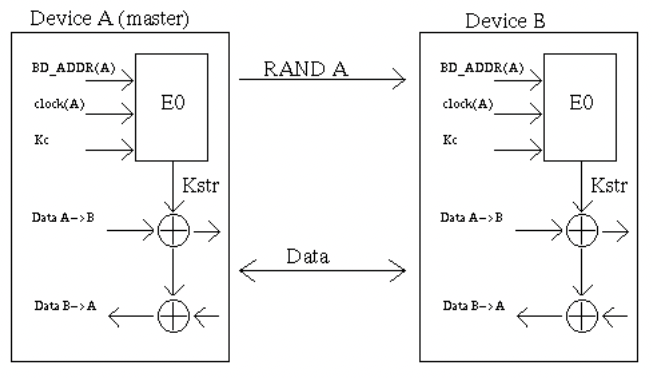
\includegraphics[width=0.5\textwidth]{images/enc.png}\hfill 
	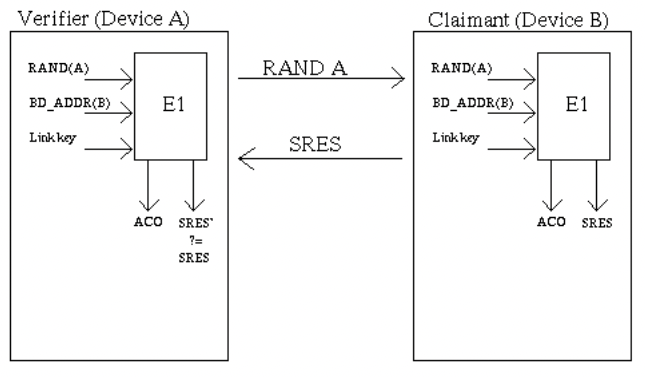
\includegraphics[width=0.5\textwidth]{images/auth.png}
	\caption{(a) Encryption process \quad (b) Authentication process (images from \cite{vainio2000bluetooth}).}
	\label{blusec}
\end{figure}

Secondly, Apple, in \cite{aps}, defines the enhancements made to provide greater security to Bluetooth and BLE; from \cite{aps} on page 172:`` The Bluetooth security model for both versions includes the following distinct security features:
\begin{itemize}
  \item Pairing: The process for creating one or more shared secret keys.
  \item Bonding: The act of storing the keys created during pairing for use in subsequent connections to form a trusted device pair.
  \item Authentication: Verifying that the two devices have the same keys.
  \item Encryption: Message confidentiality.
  \item Message integrity: Protection against message forgeries.
  \item Secure Simple Pairing: Protection against passive eavesdropping and protection against
  man-in-the-middle attacks."
\end{itemize}
According to \cite{aps}, Apple has also added two features for BLE: Address Randomization and Cross-Transport Key Derivation.

\paragraph{Address Randomization.}\label{random} According to \cite{aps}, the BLE address of an Apple device is changed frequently to prevent traffic from being analysed and to ensure that it cannot be tracked. This is obtained through a technique called \textit{Address Randomization} that allows the device to change its \textit{public} BLE address frequently. Only known devices can resolve the \textit{private} BLE address, as they require possession of the resolution key, which is exchanged between the two devices during the pairing phase.

\paragraph{Cross-Transport Key Derivation.}
Originally, the link keys of BLE and Bluetooth were independent of each other. With this functionality (introduced in the Bluetooth standard), it is possible to derive a BLE link key from a Bluetooth link key and vice versa. This reduces the number of pairings required between two devices, which increases convenience and security, according to \cite{antonioli2022blurtooth}.

\subsubsection{UWB}\label{sec:uwb}
\subsubsubsection{Overview}
In the field of wireless communication technologies, UWB works with extremely low-power, short-duration pulses that cover a broad spectrum and lead to increased precision in distance measurement. This enables high data transmission rates and precise positioning over a wide frequency range, typically several gigahertz. Originally designed for military and radar applications, it has gradually conquered various sectors and can be found particularly in consumer electronics, healthcare, automotive systems and the Internet of Things (IoT).

According to \cite{article}, one advantage of UWB technology is its ability to provide accurate, real-time tracking thanks to techniques such as Time-of-Flight (ToF)\footnote{From \cite{tof}, ``Time of flight is the measurement of time taken to travel a distance in order to determine distance, speed, or properties of the medium".}, Time Difference of Arrival (TDoA)\footnote{From \cite{tdoa}, ``TDoA is a positioning methodology that determines the difference between the time-of-arrival (ToA) of radio signals. TDoA is used in a real-time location system (RTLS) to accurately calculate the location"} and Two-Way Ranging (TWR)\footnote{From \cite{twr}, ``The Two Way Ranging method determines the Time of Flight of the UWB RF signal and then calculates the distance between the nodes by multiplying the time by the speed of light."}. According to \cite{article}, the range error can be up to 58 mm.

Due to the wide use of the spectrum, UWB can peacefully coexist with other wireless technologies and send huge amounts of data quickly. It also has a shorter range due to the wide radio bandwidth it utilizes (according to \cite{Zafar2019}, ``U1 chip can emit data using two frequencies: 6.24 GHz and 8.2368 GHz. The FCC has allocated ultrawideband a spectrum starting from 3.1 GHz to 10.6 GHz."). To overcome this problem, we can use a \textit{MIMO} (multiple-input and multiple-output) type antenna to increase the range of UWB; this kind of equipment can be integrated into our everyday devices due to its small size.

According to \cite{aps}, ``Apple-designed U1 chip uses UWB technology for spatial awareness, allowing iPhone 11, iPhone 11 Pro and iPhone 11 Pro Max or later iPhone models to precisely locate other U1-equipped Apple devices". This means that when two U1 devices come close to each other, they both start to measure their exact distance with ToF. According to IEEE 802.15.4a \cite{5394030}, the range of visibility of UWB is about 200 meters. This means that we can use this technology to locate items that are very close to us and those that are relatively far away.

It is important to recognize the differences between BLE and UWB. The former allows the detection of a device, but cannot accurately measure its position as it depends on the range of the device. UWB, on the other hand, enables precise localization of the device by measuring its position based on the time interval between when it leaves point A and when the signal arrives at point B.
Table \ref{tableu} represents the main differences between the two technologies, the data is taken from \cite{encstore}.
\begin{table}[h] 
\caption{BLE-UWB comparison.}
  \centering
  
    \begin{tabular}{l|l|l|}
      \cline{2-3}
      {}                               & {\textbf{UWB}}                & { \textbf{Bluetooth (BLE Beacons)}} \\ \hline
      \multicolumn{1}{|l|}{{  \textbf{Battery}}}  & {  Low consumption}             & {  Low consumption}                  \\ \hline
      \multicolumn{1}{|l|}{{  \textbf{Data Rate}}}  & { 1 Gbps }             & { 2 Mbps }                  \\ \hline
      \multicolumn{1}{|l|}{{  \textbf{Range}}}    & {  up to 200 meters} & {  up to 100 meters}       \\ \hline
      \multicolumn{1}{|l|}{{  \textbf{Accuracy}}} & {  10 centimeters} & {  up to a meter}                    \\ \hline
      \multicolumn{1}{|l|}{{  \textbf{Cost}}}     & {  Low}                         & {Depend on the context }                              \\ \hline
    \end{tabular}
    \label{tableu}
  \end{table}

\subsubsubsection{Security Analysis}
The fact that UWB pulses are resistant to the multipath effect\footnote{From \cite{Figueroa2022}: ``Multipath interference occurs when a signal from a transmitter arrives at a receiver via two or more routes; typically there is a direct path plus a number of indirect paths caused by reflections".} is one of its key characteristics. This occurs when radio waves are reflected or refracted by artificial or natural objects near the primary signal channel, causing the signal to reach the receiver via many paths. Positioning accuracy is improved by immunity to the multipath effect, particularly when compared to other technologies that are more vulnerable. Moreover, UWB's resilience to jamming and narrowband fading makes it a particularly reliable technology choice, even when several UWB systems are being used at once.

Another important aspect to consider is the resistance to Relay Attacks, which is a vulnerability of the majority of signal-based architectures; we will present a concrete example taken from \cite{Global_2020}. In this attack, the goal is to trick a car into thinking the key and owner are close by using two people with hacking devices. The first relays signals from the car to the second thief, who transmits the signal to the house. The key responds, allowing entry into the car. The relay attack intercepts and amplifies wireless signals used to unlock the door and start the car, despite the key's distance. With UWB, that would not be possible due to its working scheme: to ensure the car doesn't have to make assumptions, rapid measurements are utilized to establish distance very precisely. Any attempt to relay attack or intercept the UWB signal will merely cause the answering device's acknowledgement signals to arrive later, indicating to the car that the real key is actually farther away. The car's presumption is replaced with assurance when using UWB, which greatly increases the security of the passive keyless entry system.

The implemented security measures, taken by Apple, are the following: MAC address randomisation and frame sequence number randomisation \cite{aps}.

\paragraph{MAC address randomisation.}
This functionality is very similar to that discussed in \ref{random}, with the aim of hiding the MAC address of the device. In \cite{aps}, it is explained that the randomization procedure used for UWB is the same as the one used for Wi-Fi. During a scan, the device randomizes its MAC address to prevent anyone from sniffing the traffic to analyze the device's behavior. Once the device is connected to a network, it always displays the same (randomized) MAC address, which changes when the session ends. This provides protection against the visibility of malicious individuals attempting to spy on the traffic for malicious purposes.

\paragraph{Frame sequence number randomisation.}
This feature provides that every time the device randomizes its MAC address (after a scan or disconnection), the sequence number of its packets is also randomized; this addition increases privacy and also prevents the possibility of replay attacks.

We will now analyze the architecture of this product; the information was reverse engineered by Adam Catley in \cite{reverse}. We will cover both the hardware and software aspects of this type of device.

\subsection{Hardware Analysis}\label{hw}
As for the hardware part, an important aspect comes to light: all the components used, apart from Apple's U1 UWB chip, are off-the-shelf, as we can see in Figure \ref{img:pcb}.
Each AirTag has three antennas: one for BLE operating at 2.4 GHz, one for NFC at 13.56 MHz and one for UWB at 6.5-8 GHz.
We have a plastic case that works as a membrane and it is glued to the voice coil. When power is applied to the coil, the fixed magnet moves back and forth, creating a sound that acts as a speaker.
When movement is detected, the speaker emits a loud beep for up to 20 seconds after it has been separated from its owner for three days. It then remains silent for the next six hours before listening for movements again.
\begin{figure}[ht]
	\centering
	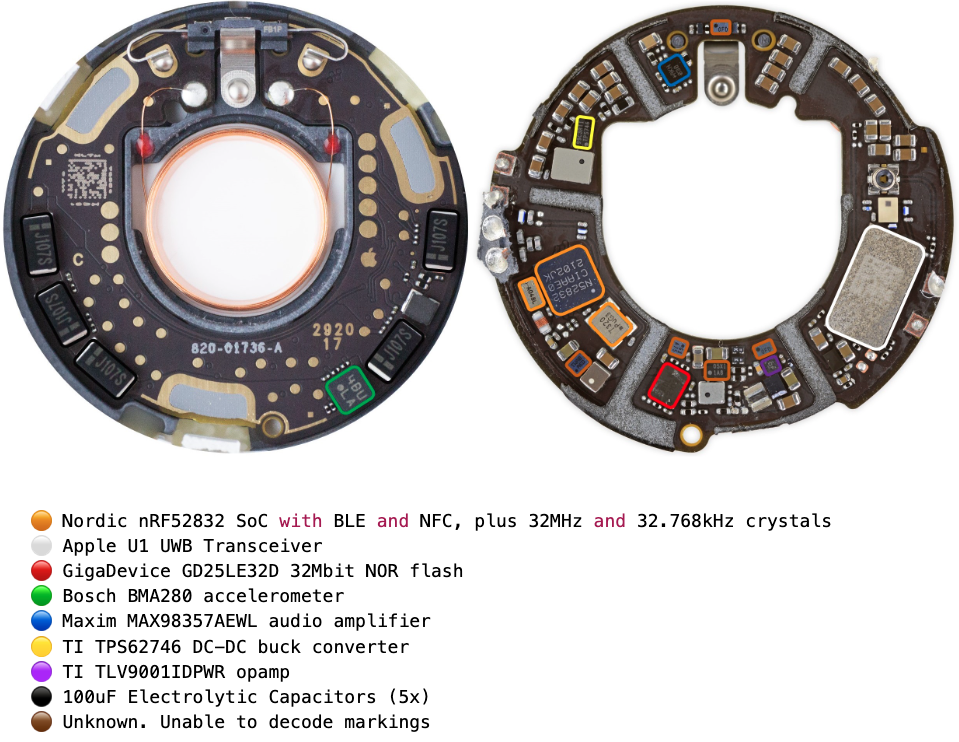
\includegraphics[width=\textwidth]{images/pcb.png}
	\caption{PCB overview (image from \cite{reverse}). }
	\label{img:pcb}
\end{figure}

\subsection{Software Analysis}\label{sec:beacons}
As for the software part, we will present information taken from \cite{reverse}: ``There are various states in which AirTag can be; we will now quickly present all of them.
\begin{itemize}
  \item \textit{Not registered}: When the AirTag is brand new, has been reset, or has been removed from the FindMy network. Waits to be connected to while advertising itself every 33ms.
  \item \textit{Initialisation}: The AirTag is being registered to an Apple ID and a public/private key pair is generated and shared between the AirTag and the connected iOS device.
  \item \textit{Connected}: The owner’s device is in range. No broadcasts occur.
  \item \textit{Disconnected}: The owner’s device is out of range. Broadcasts identity every 2000 ms.
  \item \textit{Out of sync}: Happens when an AirTag reboots while separated from its owner’s device. Acts like Disconnected but absolute time is lost so events are relative to time since power-up. Identity resets to initial value.
  \item \textit{Lost}: Occurs 3 days after Disconnected or Out of sync begin. Moves to Waiting for motion every 6 hours.
  \item \textit{Waiting for motion}: Samples the accelerometer every 10 seconds until motion is detected.
  \item \textit{Sound alert}: A command to play a noise is received from either a connected device or by detecting motion. Lasts a maximum of 20 seconds.
  \item \textit{Precision finding}: Triggered by the owner’s device while in Connected. Is overridden by Sound alert."
\end{itemize}
As we will see in Section \ref{hw}, thanks to the NFC antenna, the finder can identify the owner of an AirTag even if it has an Android device. Depending on its current status, the tag carries a URL that uniquely identifies the AirTag. It can only be read if the AirTag is switched on (which means that the battery is sufficiently charged). The URL is linked to several parameters that are used to identify the device; we will briefly introduce them. All the following parameters are fixed for a single unit, even after power cycles, long runtimes, resets and modes. From \cite{reverse}, ``
\begin{itemize}
  \item \textit{pid}: product ID for AirTag.
  \item \textit{b}: something related to the battery.
  \item \textit{pt}: UWB Precision Tracking version.
  \item \textit{fv}: firmware version.
  \item \textit{dg}: something related to diagnostic.
  \item \textit{z}: unknown.
  \item \textit{bt}: Bluetooth address; will be present only when Unregistered.
  \item \textit{st}: serial number of the tag (the one printed on the device under the battery); will be present only when Unregistered.
  \item \textit{bp}: Bluetooth protocol version; will be present only when Unregistered."
\end{itemize}
In the \textbf{Unregistered} state, the saved URL has the following format:
\url{https://found.apple.com/airtag?pid=5500&b=00&pt=004c&fv=00100e10&dg=00&z=00&bt=A0B1C2D3E4F5&sr=ABCDEF123456&bp=0015}

According to \cite{reverse},
once the device is registered, ``The parameters \textit{bt, sr, bp} will be removed and replaced with a single anonymous identifier \textit{pi}, which is the only parameter that changes at least every 15 minutes when the Bluetooth address and/or the advertising data change". Probably, it is the P-224 $p_i$ presented in \ref{keys} or the SHA-224 of it. 

The device works according to a schedule designed to optimize its functionality:
every day at 4:00 am , it updates its BLE address and public key to ensure secure communication channels.
Advertisement data is updated every 15 minutes to ensure that nearby devices receive the most up-to-date information.
Should it be separated from its owner's device for three days, the device switches to a lost mode and activates specific features to help with recovery.
When the device is in this mode and detects movement, it emits a sound every 6 hours to alert people in the vicinity.
To conserve energy while remaining responsive, the accelerometer is sampled every 10 seconds while waiting for movement. Once motion is detected, the sampling frequency increases to every 0.5 seconds for 20 seconds, providing detailed tracking data.
When it is not near the owner, the device sends BLE advertising signals every 2 seconds to increase its recognizability.
Finally, in close proximity to its propietor’s device, the tag establishes a BLE connection interval of 1 second to ensure efficient communication and responsiveness.

\subsection{Security Analysis}\label{sec}
Security-wise, from \cite{reverse} it has emerged that no security checks are performed on the device during its operations; in fact, none of the data in the AirTag is protected from tampering or disclosure.
\subsubsection{Vulnerabilities}\label{sec:vuln}
We will present some vulnerabilities that have been found by Adam Catley in \cite{reverse}; Table \ref{vuln} resumes them.
\paragraph{Exploitable voltage levels.}
The Nordic nRF52832 has the function Access Port Protection \cite{nordicsemi} that is used to prevent external parties from reading the internal memory and to limit access to the Debug Port via SWD\footnote{From \cite{Oberli_2019}, ``SWD is a standard for debugging and accessing microprocessor registers. This protocol has been in use for many years and is still in use today."}; however, according to \cite{side}, side channel attacks are effective against this mechanism, more specifically voltage glitching. Consequentially, ``It would be possible to disable other privacy features that Apple advertises, extract Bluetooth pairing keys to connect to the owner’s phone, or run completely custom firmware", from \cite{reverse}. In this case, if an attacker is able to use voltage glitching to inject a modified firmware, maybe he can use it to track the owner and it will not be discovered since the anti-stalking countermeasures presented in \ref{countermeasures} do not work with personal objects. 
To ensure protection against voltage glitching attacks, it is necessary to implement a detector directly on the circuit that can detect when the voltage levels are being manipulated. INVIA's Voltage Glitch Detector IP ``detects positive and negative supply voltage glitches, and has a slope detection range between 100 MV/s and 2 GV/s", according to \cite{voltage}.

\paragraph{Insecure Storage.}All the information saved in the GD25LE32D 32Mbit NOR flash is clear, as we can see in \cite{tweet}; moreover, the nRF52832 has no encryption function. In this case, we do not know if it is a real vulnerability because we do not know whether the FindMy private key-pair is stored in the AirTag. However, an attacker can easily read all the information stored in the device and this behavior can be exploited (perhaps in the future) to inject malicious data into the AirTag or read sensible information. To prevent this, we can implement encryption via software or hardware; typically, on small devices, it is better to use dedicated hardware circuits to encrypt the data.

\paragraph{Unathenticated transmission.}To identify an AirTag we need its public key, which is transmitted via BLE advertising packets; this identification does not require authentication. These IDs can be recorded and replayed by any nearby BLE device to mimic the appearance of the real AirTag. Suppose a malicious actor obtains a BLE device and records the public key of the sender; once power is removed from the AirTag, the attacker can send BLE packets with the AirTag's public key to spoof the AirTag's location without a battery. In this case, the AirTag is exploited to steal the owner's personal belongings (example from \cite{reverse}). To avoid this, Apple can use authenticated encryption. For example, we can use GCM, which in addition to authenticated encryption (confidentiality and authentication) also provides the ability to verify the authenticity and integrity of extra authenticated data (AAD) provided in plain text. Further details can be found in \cite{gcm}.

\begin{table}[h] 
  \caption{Vulnerabilities.}
  \centering
  \begin{tabularx}{\textwidth}{|X|X|X|}
    \hline
    \textbf{Vulnerability}      & \textbf{Possible attack} & \textbf{Countermeasure}             \\ \hline
    Exploitable voltage levels  & Side-channel attack      & Use detector         \\ \hline
    Insecure storage            & Memory-reading attack    & Implement hardware encryption \\ \hline
    Unauthenticated transmission & Replay attack            & Implement authenticated encryption                     \\ \hline
  \end{tabularx}
  \label{vuln}
\end{table}

\subsubsection{Anti-stalking countermeasures}\label{countermeasures}
An important aspect that has emerged in connection with AirTags is the problem of stalking. Stalking with AirTags refers to the potential misuse of Apple's AirTag tracking devices to monitor and track individuals without their consent; these small devices are designed to help users find misplaced items. However, due to their small size and long battery life, AirTags can also be used for nefarious purposes, such as stalking. A person could secretly place an AirTag in another person's belongings and then use the Find My app to monitor their movements in real time. Because AirTags are designed to be difficult to detect, the victim may not realize they are being tracked for an extended period of time.

Apple has taken measures to prevent the misuse of AirTags. These include alerts and notifications when an unknown AirTag is detected near a user's device, as well as features such as Precision Finding, which allows users to track down unwanted AirTags. The first line of defense in the event that someone attaches an AirTag to a victim's belongings could be an alert on the iPhone indicating the presence of a foreign AirTag. Apple has designed the connection between iPhone and AirTag so that this happens in two ways: either when you arrive at the location that your iPhone's machine learning intelligence has recognized as home (or when you manually record it as home) or after the AirTag has stayed with you for a certain ``uninterrupted" period of time that Apple deems sufficient to be considered abnormal. That seems perfect. However, if the victim has a non-Apple device, such as an Android phone, this could be a problem. To prevent this, Google and Apple collaborated to develop Unknow Tracker Alerts, a feature that was announced during the opening presentation of Google I/O 2023.

In the paper \cite{shafqat2023track}, an experiment was conducted in which the payload of the beacon sent by the AirTag was successfully modified so that it appeared as an iPhone and thus could not be recognized as a tracking device. As a result, no tracking notifications were triggered.

An important factor is that AirTags can emit sounds if they are disconnected from the owner's devices for an extended period of time. In this way, a victim of a stalking attempt can hear the sound emitted by the device and recognize that it is being tracked. More specifically, the acoustic warnings start three days after the separation. Even in this case, once the tag detects movement, it will emit a sound for about 20 seconds, followed by at least 6 hours of silence (even if further movement is detected). The issue with this feature is that 20 seconds of sound followed by 6 hours of silence may be ineffective if the victim is in a noisy environment and cannot hear the sounds emitted by the device. In addition, during the first three days of silence, the attacker can study the victim's movements undisturbed without him being aware of it. According to \cite{server}, ``The frequency and duration of sounds can be adjusted from the Apple server side", meaning that Apple can increase both to avoid situations where the victim cannot hear the sounds.

Despite these safety precautions, the possibility of AirTags being used for stalking remains a concern; one problem is that the voice coil can be disconnected without disassembly. The resulting problem is that an AirTag can function normally without the voice coil. So if it is used for stalking, it is difficult for a user without an Apple device to detect its presence if it is well hidden.

\subsection{Patents} 
There are several patents related to AirTags; illustrations and information from these patents are presented below. Patent US2020028424 (Wirelessly locatable tag) \cite{Perkins_Sano_Walton_Wang_Werner_Ashcroft_De_Hunter_Kim_Crosby_Jung_Schaevitz_Avendal_Da_Di_Nath_Papantonis_Graham_Thompson_Copeland_Ely_2022} first describes the structure of the tag, as shown in Figures \ref{img:br1} and \ref{img:br2}, and then outlines the abstract requirements for the components that this device must contain. 

Other patents similar to the one just mentioned are:
\begin{itemize}
\item US20220004834A1 (Antenna assembly for a wirelessly locatable tag) \cite{Perkins_Avendal_Da_Di_Nath_Papantonis_Schaevitz_Werner_2022}, which provides information on the arrangement of the antenna.
\item US11659916B2 (Mounting base for a wirelessly locatable tag) \cite{Perkins_Thompson_2023}, which describes the construction of the mounting base for the tag.
\item US20200333421A1 (Fastener with a constrained retention ring) \cite{Perkins_De_Hunter_2020}, which describes the construction of a generic holder for the tag.
\item US20200272221A1 (Multi-Interface transponder device - power management) \cite{Foster_Nilsen_Puskarich_2020}, which describes the various states in which a positioning tag can be; they are shown in Figure \ref{img:br3}.
\item US20240073648A1 (Tracking Systems with Electronic Devices and Tags) \cite{Puskarich_2024}, which describes the need for communication circuits that enable communication between tags and devices.
\end{itemize}
Many illustrations are included in all previous patents.

\begin{figure}[]
	\centering
	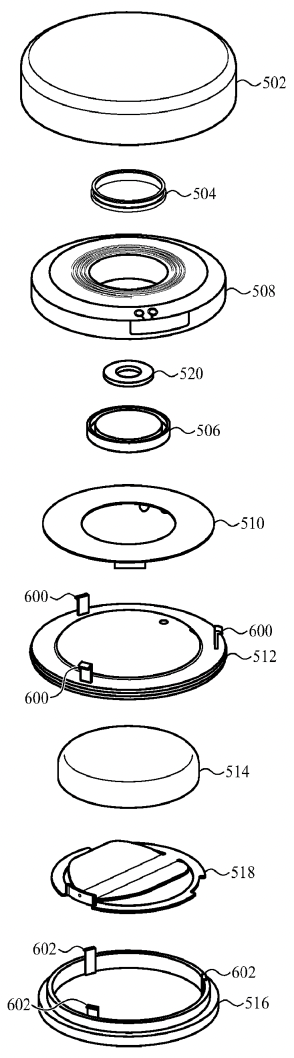
\includegraphics[width=0.5\textwidth]{images/br1 struttura.png}
	\caption{Tag composition (image from \cite{Perkins_Sano_Walton_Wang_Werner_Ashcroft_De_Hunter_Kim_Crosby_Jung_Schaevitz_Avendal_Da_Di_Nath_Papantonis_Graham_Thompson_Copeland_Ely_2022}). }
	\label{img:br1}
\end{figure}

\begin{figure}[]
	\centering
	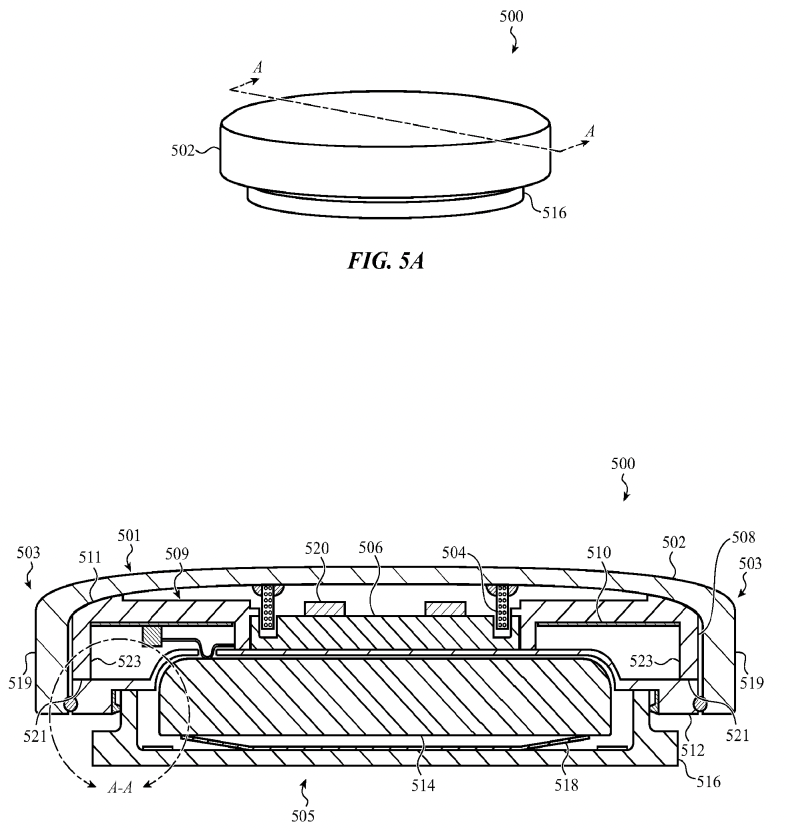
\includegraphics[width=\textwidth]{images/br1 s2.png}
	\caption{Tag sectional drawing (image from \cite{Perkins_Sano_Walton_Wang_Werner_Ashcroft_De_Hunter_Kim_Crosby_Jung_Schaevitz_Avendal_Da_Di_Nath_Papantonis_Graham_Thompson_Copeland_Ely_2022}). }
	\label{img:br2}
\end{figure}

\begin{figure}[]
	\centering
	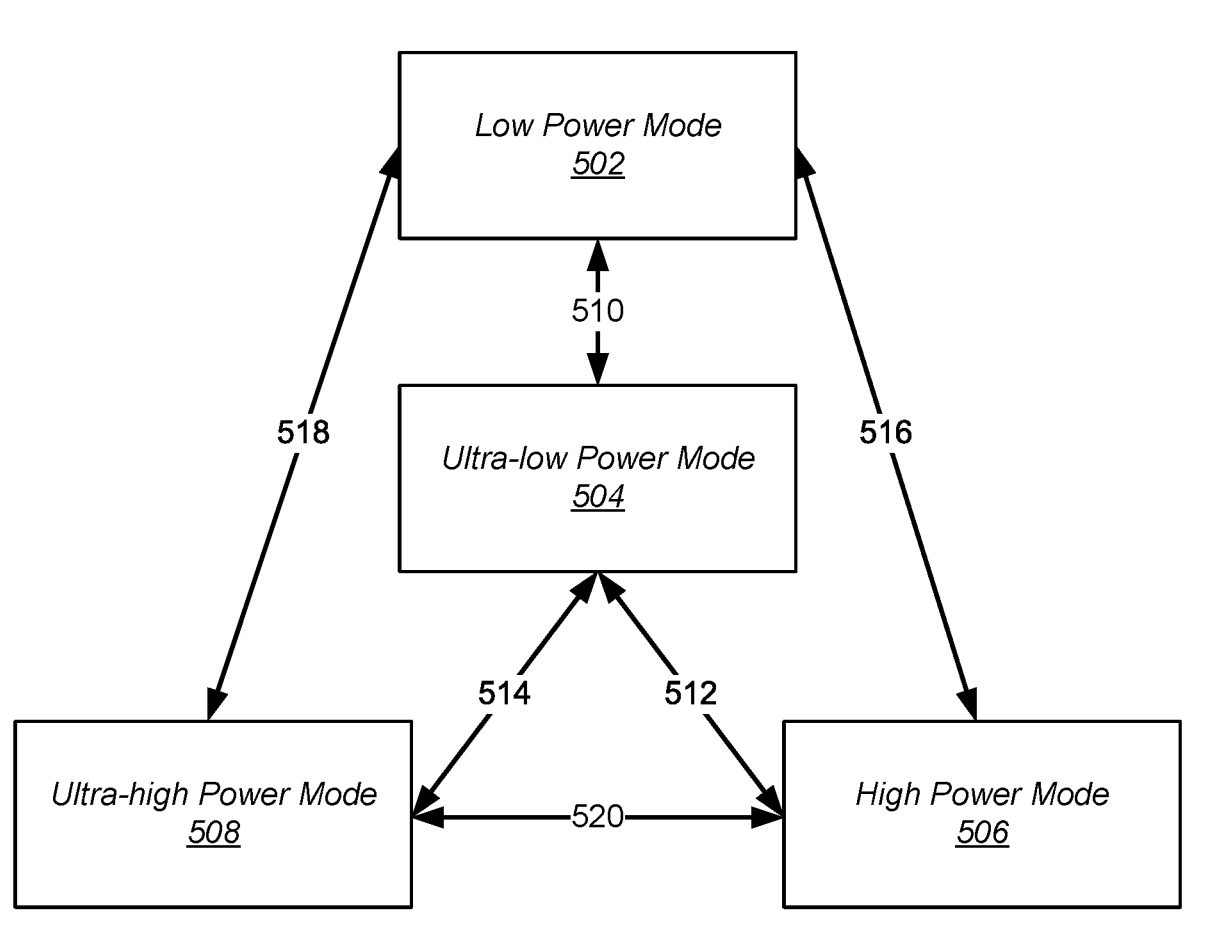
\includegraphics[width=0.8\textwidth]{images/br3.png}
	\caption{State diagram that represents power modes of a tag (image from \cite{Foster_Nilsen_Puskarich_2020}). }
	\label{img:br3}
\end{figure}


\section{FindMy Network}\label{sec:find}
\subsection{Overview}
Apple has developed the technology known as the FindMy network to help consumers find compatible third-party accessories, such as Apple AirTags, as well as their Apple devices, including iPhones, iPads, Macs, and AirPods. Utilizing UWB and BLE technologies, the FindMy network enables accurate and instant location tracking.

Apple merged the Find My Friends and Find My iPhone applications into a single one called \textit{Find My}, allowing users to locate everything they need in one place. Apple then expanded the Find My app, adding functionalities such as monitoring when an iPhone is disconnected, when it is turned off and when it has been erased.

Sections of the app are located at the bottom. \textit{People} is located on the left and represents friends location (they have to share it in order to be visible), while personal belongings, including Bluetooth goods with Find My functionality and AirTags, are located in the center; finally, on the right, there's a \textit{Me} tab with all of the owner's settings and info, as we can see in Figure \ref{findmy2}.

There are several useful features within this app, we present some examples from \cite{Clover_2022}:
\begin{itemize}
  \item \textit{Separation alerts}: You will be notified if you accidentally leave behind an Apple device, an AirTagged item, or a third-party device that has Find My features enabled.
  \item \textit{Locating friends and sharing location}: This feature allows you to share your location with friends or family members so they can view it when needed. A useful aspect of this feature is that you can also use it to monitor your children or people with certain orientation issues to help them if they get lost.
  \item \textit{Locating devices without connection}: This feature is very useful as it allows you to locate offline devices via the FindMy network. Essentially, a lost device uses BLE to send beacon packets to nearby Apple devices, which then send the encrypted location to the owner’s iCloud account. As we will see later, some devices can be tracked even without a battery charge, i.e. when the device is switched off.
  \item \textit{Anti-stalking measures}: This feature helps prevent a malicious person from secretly placing a device belonging to a FindMy network in your belongings to track your location in real time, using your device to upload its location. If your device receives multiple BLE beacons from a nearby device, you will be notified that you may be tracked by a device and asked if you want to disable location sharing. We will also return to this following the studies in \cite{airguard}.
  \item \textit{Precision finding}: This feature requires the presence of the U1 chip, which uses UWB technology to locate another device equipped with the same chip. It is very useful for the precise location of AirTags, which are often attached to items that we frequently lose. The range of this technology is, as already mentioned, limited to UWB.
\end{itemize}

\begin{figure}[t]
	\centering
	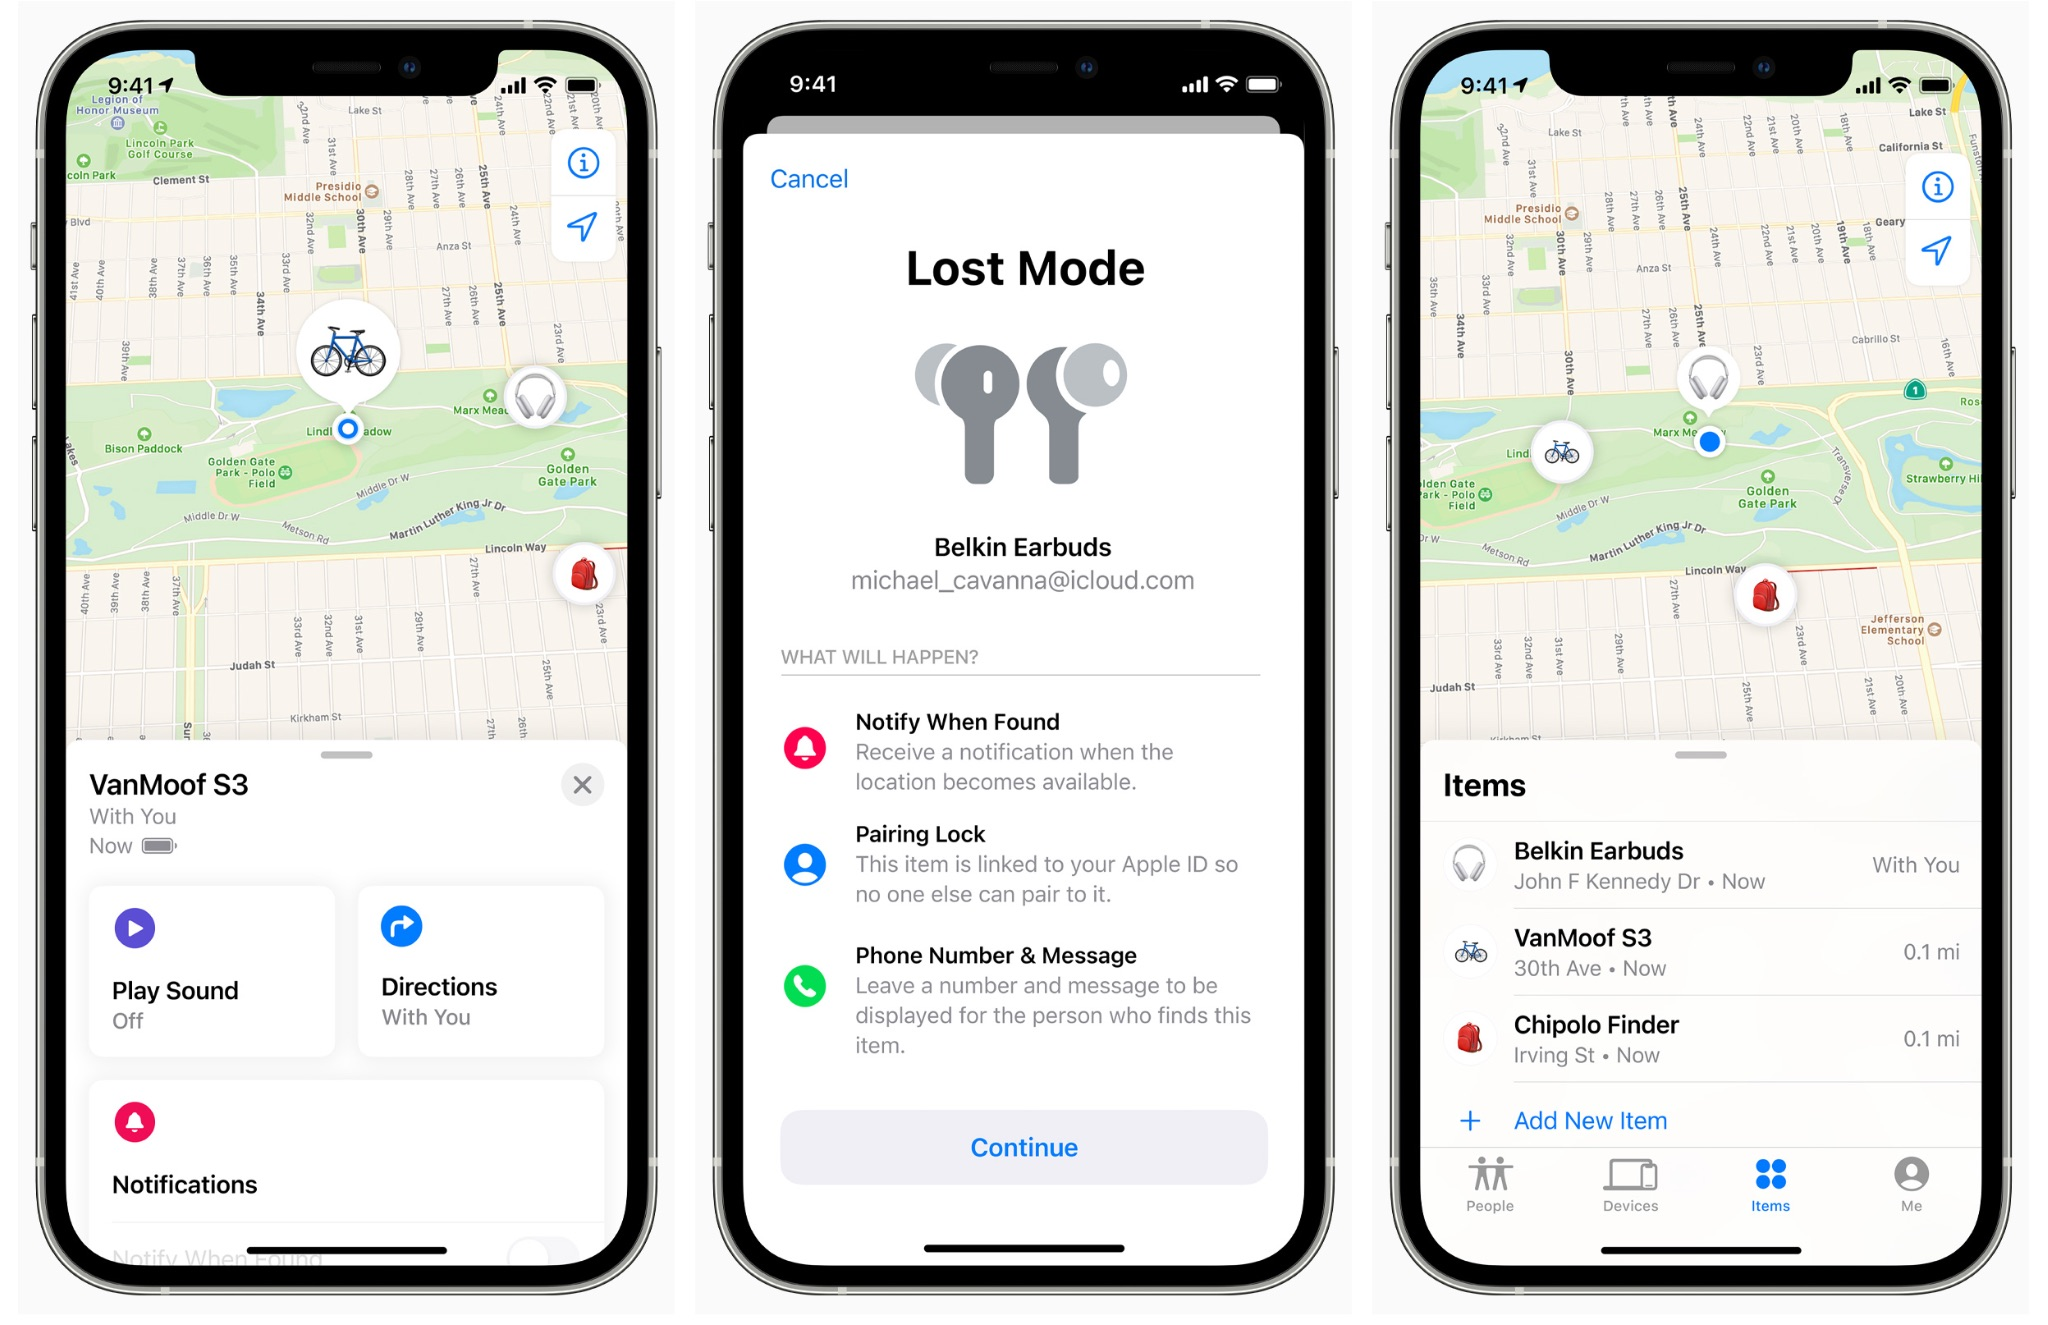
\includegraphics[width=.9\textwidth]{images/findmy.jpg}
	\caption{FindMy screenshots (images from \cite{findmyscreen}).}
	\label{findmy2}
\end{figure}

\subsection{Functioning}
%As for the functioning, we will use the content of \cite{Mayo_2021,Itani_2021,Clover_2022,OBoyle_2021} to describe the entire process. 
Now, we will describe the entire functioning process. First, the products must be registered in the application. If it is an item that is not an accessory, it is automatically added to the \textit{Devices} section. If it is an accessory, such as AirTag, it will be added to the \textit{Items} section.

Now devices should be locatable from the map; in the case of a nearby AirTag it is also possible to use the \textit{Precision finding} to locate the item using the U1 chip, as shown in Figure \ref{findmy1}. As always, Apple has created an excellent graphical interface for its features; Precision Finding, for instance, uses several components. From \cite{OBoyle_2021}: ``The technology fuses input from the iPhone's camera, ARKit, accelerometer and gyroscope in order to guide the user to their AirTag using a combination of sound, haptics, and visual feedback." 

\begin{figure}[t]
	\centering
	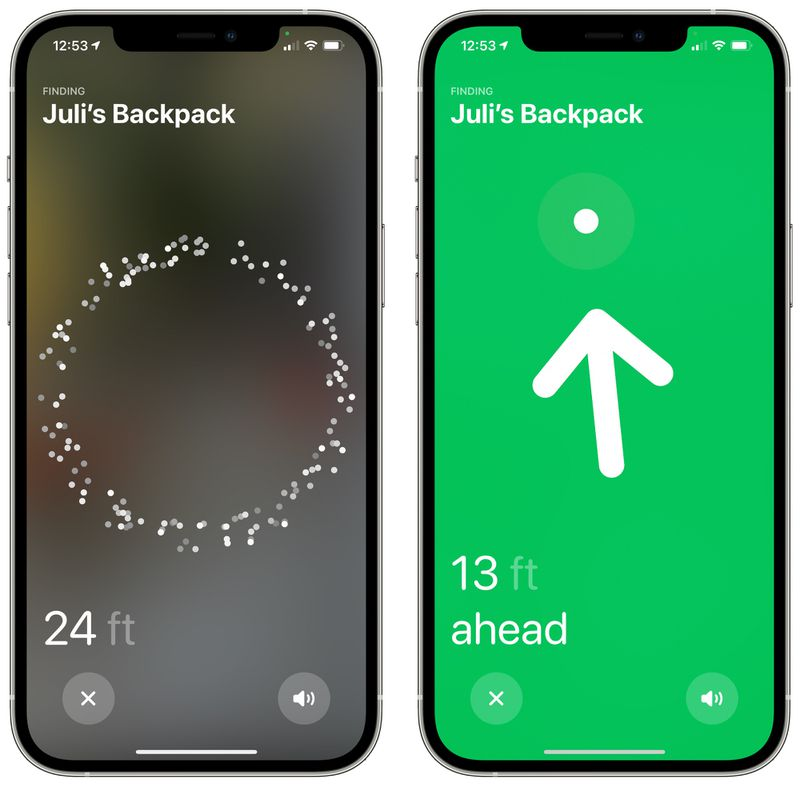
\includegraphics[width=.6\textwidth]{images/airtag-precision-finding-2.jpg}
	\caption{Precision Finding.}
	\label{findmy1}
\end{figure}

In the event of a stolen device, it is possible to activate \textit{Lost Mode} at any time. As soon as the iPhone is detected, a notification is sent, i.e. if the phone is connected to a network or via BLE to other Apple devices, the owner will receive a message from FindMy with the location of the device. In addition, all cards registered in Apple Pay are temporarily disabled in this mode.

This technology already seems to be quite useful, but how can a switched off device be localized? If it is equipped with U1, its Bluetooth is activated and its iOS version is at least 15, it can be located even when it is switched off, as it works like an AirTag. That seems very useful. But what about other devices, like Macbooks? Since Apple has not commented on this issue, the author did some tests and found that even high spec devices do not have the U1 chip and are therefore not locatable when turned off.

Like other devices registered with FindMy, AirTags can be located by other Apple devices in the same way as previously written. As we will see in Section \ref{sec:beacons}, once an AirTag moves out of close range of the owner's other devices, it will begin sending BLE beacons to be identified and located on FindMy. The only way to stop an AirTag from being fully detectable is to remove the CR2032 coin battery (or when it fully discharges).

\subsection{Security Analysis}
In this section, we will analyze the security measures implemented in FindMy to increase the security of the architecture.
\subsubsection{Preliminary definitions}
First, we will define some terms from \cite{whocanfind}:
\begin{itemize}
  \item \textit{Owner Devices}: Apple devices that are owned by the user and can be located; see \cite{Apple} for the full list of discoverable devices. You can view the location of all your devices in the FindMy section of your iCloud account.
  \item \textit{Lost Devices}: There can be two types of Apple devices: devices and accessories (according to \cite{whocanfind}). The former (which appear in the Devices section of FindMy) are marked as lost if they lose their Internet connection, while the latter (which appear in the Items section) are marked as missing if they lose connection to all of the owner’s Apple devices. As we will see in Section \ref{sec:crypto}, these devices will start sending BLE beacons to be recognized by other Apple devices.
  \item \textit{Finder Devices}: Apple devices that are able to locate lost devices; a GPS module is required to be a finder.
  \item \textit{Apple’s Servers}: They are used to store all the location reports sent by the different Finder devices and only the respective parties can access and download them locally. All information is encrypted and only those who have the private key can access it, namely the owners of the devices involved.
\end{itemize}
\subsubsection{Workflow}
An Apple device or accessory that enters the Lost state will begin broadcasting BLE beacons that can be detected by nearby Apple Finder devices. Once a beacon is detected, the Finder device creates a packet with information about the lost device and uploads it to iCloud. An example of the previous workflow is shown in Figure \ref{process}.

\begin{figure}[]
	\centering
	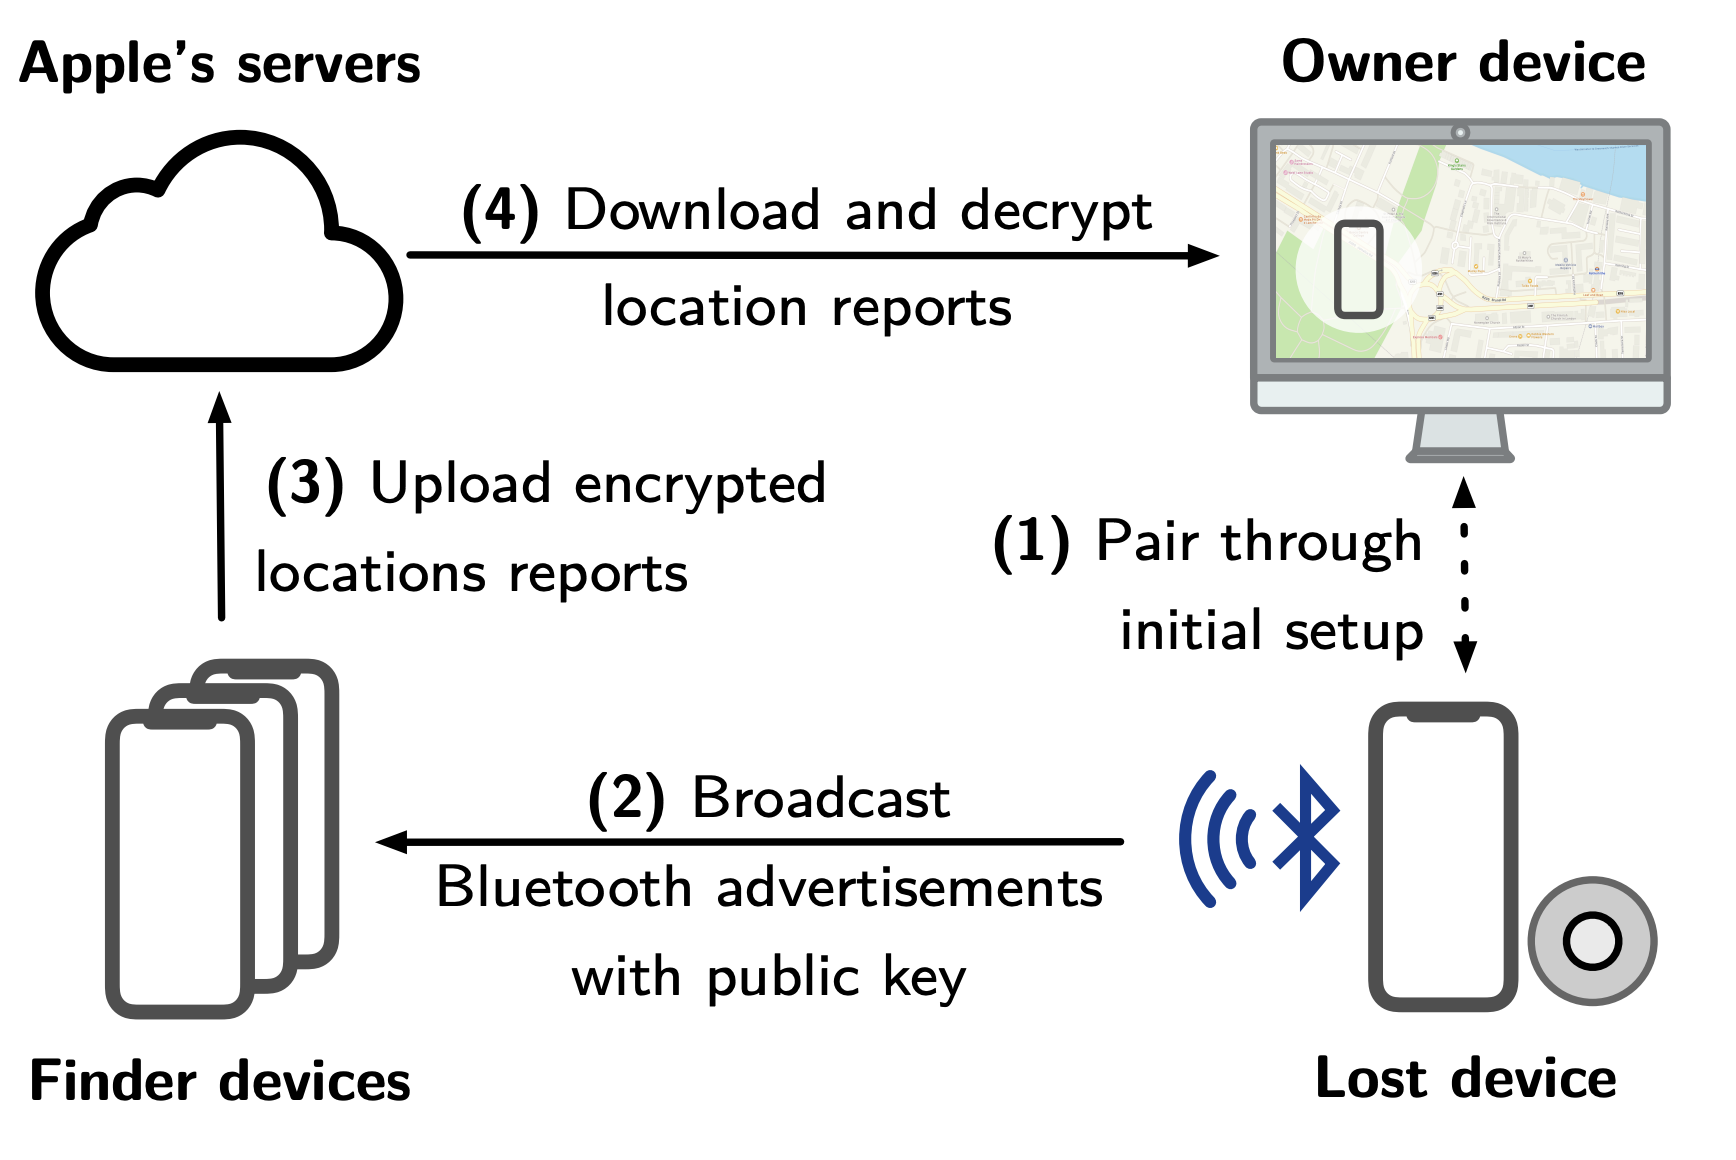
\includegraphics[width=.5\textwidth]{images/process.png}
	\caption{FindMy workflow (image from \cite{whocanfind}).}
	\label{process}
\end{figure}
All Finders scan for FindMy beacons (if the option is enabled in the settings). More specifically, this kind of device creates an encrypted location report and uploads it to the Apple servers as soon as they receive a beacon in FindMy advertising format. They probably consume less energy and bandwidth because they collect the reports over time and transmit them regularly in batches. The evaluation conducted in \cite{whocanfind} discovered that ``The median time from generating to uploading a location report is 26 minutes. The delay can increase to several hours if the finder device is in low power mode".

\subsubsection{Cryptography} \label{sec:crypto}
We will now delve more into the Cryptography protocols used. 
\paragraph{Advertisement keys.}\label{keys}
FindMy utilizes Elliptic Curves \cite{ec}; according to \cite{aps,whocanfind}, ``The process to generate \textit{advertisement keys} is the following:
\begin{enumerate}
  \item Each owner device generates a private/public key pair
  $(d_0, p_0)$ on the NIST $P-224$ curve and a $32$-byte symmetric key $SK_0$ that together form the master beacon key. Those keys are never sent out via BLE and are used to derive the rolling advertisement keys included in the BLE advertisements. Note that device tracking is hard since rolling keys can be deterministically derived if and only if one knows the initial input keys $(d_0, p_0)$ and $SK0$.
  \item OF iteratively calculates the advertisement keys $(d_i,p_i)$ for $i > 0$ as follows using the ANSI X.963 key derivation
  function $KDF$ \cite{ANSI} with $SHA-256$ \cite{sha} and a generator $G$ of the NIST P-224 curve:
  \begin{align}
    SK_i &= KDF(SK_{i-1},\ 'update',\ 32) \\
    (u_i, v_i) &= KDF(SK_i,\ 'diversify',\ 72) \\
    d_i &= (d_0 * u_i) + v_i \\
    p_i &= d_i * G
  \end{align}
  where Equation $(1)$ derives a new symmetric key from the last used symmetric key with 32 bytes length. Equation $(2)$ derives the so-called “anti-tracking” keys $u_i$ and $v_i$ from the new symmetric key with a length of $36$ bytes each. Finally, Eqs. $(3)$ and $(4)$ create the advertisement key pair via EC point multiplication using the anti-tracking keys and the master beacon key $d_0$".
\end{enumerate}

\paragraph{Key synchronization.}
To download and decode location information, the advertisement keys must be accessed by all owner devices. In order to synchronize the master beacon keys, FindMy uses iCloud to encrypt a property list file in the Galois/Counter mode of the Advanced Encryption Standard (AES-GCM) \cite{gcm}. The file's decryption key is kept in the iCloud keychain underneath the label “Beacon Store”.

\paragraph{Encryption.}
Each BLE beacon contains an Elliptic Curve public key $p_i$. When a finder device intercepts a beacon, it saves its location and encrypts it using the $p_i$ key; subsequently, it uploads the packet to Apple's servers.
OF uses the Elliptic Curve Integrated Encryption Scheme (ECIES), which generates a shared secret that is utilized to encrypt the report through an ephemeral key exchange (Elliptic Curve Diffie-Hellmann (ECDH)). According to \cite{whocanfind}, ``The finder’s encryption algorithm works as follows:
\begin{enumerate}
  \item Generate a new ephemeral key $(d', p')$ on the NIST P-224 curve for a received FindMy lost advertisement.
  \item Perform ECDH using the ephemeral private key $d'$ and the advertised public key $p_i$ to generate a shared secret.
  \item Derive a symmetric key with ANSI X.963 $KDF$ on the shared secret with the advertised public key as entropy and SHA-256 as the hash function.
  \item Use the first 16 bytes as the encryption key $e'$.
  \item Use the last 16 bytes as an initialization vector $IV$.
  \item Encrypt the location report under $e'$ and the $IV$ with AES-GCM. 
\end{enumerate} 
The ephemeral public key $p'$ and the authentication tag of AES-GCM are part of the uploaded message. All location reports are identified by
an id, which is a SHA-256 hash of $p_i$.", as we can see in Figure \ref{comparison}.

\paragraph{Decryption.}
For decryption, the procedure implemented is the reverse of the encryption process. From \cite{whocanfind}, ``An owner device that downloads encrypted location reports follows the inverse of the encryption procedure:
\begin{enumerate}
  \item The owner device selects the proper advertisement keys $(d_i, p_i)$ based on the hashed $p_i$ of the location report.
  \item It performs the ECDH key exchange with the finder’s ephemeral public key $p'$ and the lost device’s private key $d_i$ to compute the symmetric key $e'$ and the $IV$.
  \item Now, the owner can use $e'$ and $IV$ to decrypt the location report."
\end{enumerate}

\begin{figure}
	\centering
	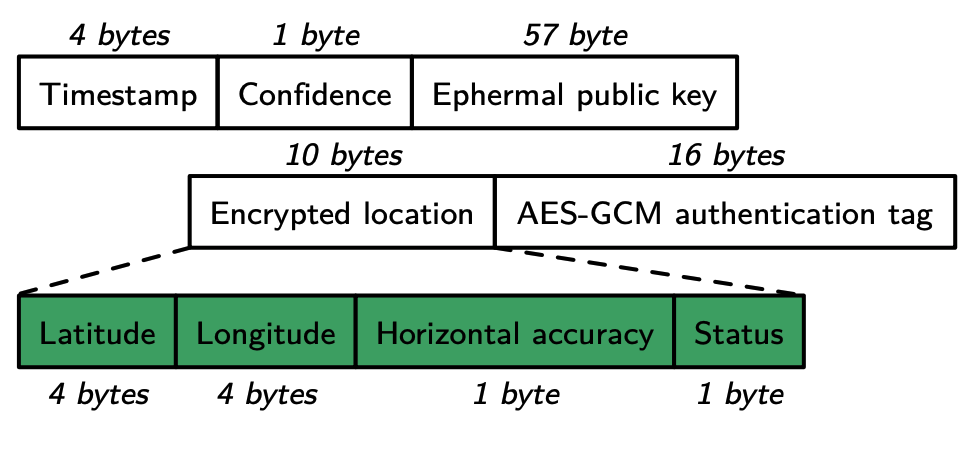
\includegraphics[width=0.5\textwidth]{images/packet.png}\hfill 
	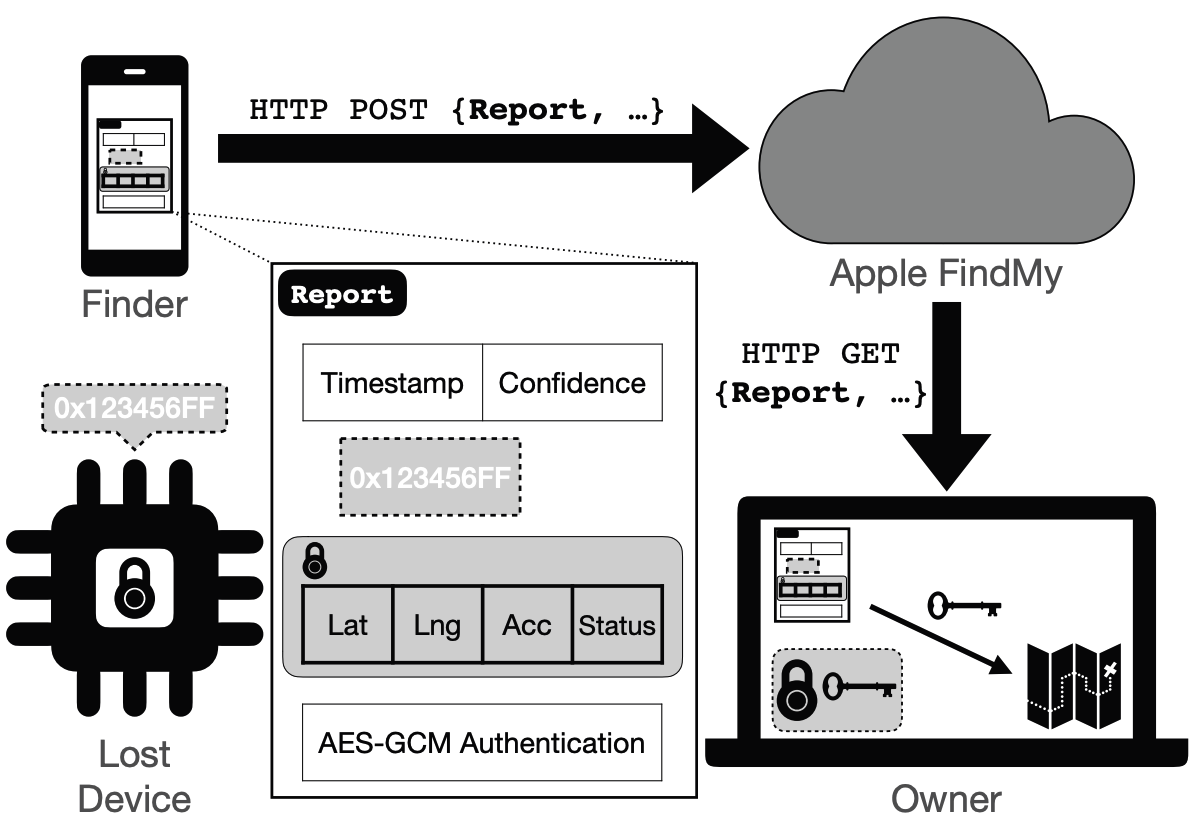
\includegraphics[width=0.5\textwidth]{images/findmysec.png}
	\caption{(a) Binary format of a location report \quad (b) Example of sent payload (images from \cite{whocanfind},\cite{airguard}).}
	\label{comparison}
\end{figure}

\subsection{Support for non-Apple accessories} 
Following WWDC 2020, support for third-party accessories within the FindMy network was announced. Apple then released the Find My Certification Assistant app in the App Store, which allows developers to test the FindMy network features on accessories developed by external companies. According to \cite{Bowe_2022}, several companies have already signed agreements with Apple to be integrated into this service. These include Belkin (with the SoundForm Freedom), Chipolo (with the One Spot tag) and VanMoof (with the X3 and S3 bicycles). In addition, Beats (owned by Apple) also supports the FindMy network with its latest products.

To check if a product under development is compatible with the FindMy network, it is necessary to be enrolled in the Made for iPhone (MFi) program \cite{MFIprogram}, which provides guidelines for developing electronic devices that can work with Apple devices.

\section{Useful applications}\label{appl}
Some useful applications include the following:
\begin{itemize}
  \item \textit{Travel}: AirTags can be beneficial for travelers. They can attach AirTags to their luggage so that they can more easily identify and track their luggage while traveling. For example, for a tourist who has just landed from a trip and is eager to pick up their luggage, waiting at the baggage carousel can be frustrating. If their luggage is tagged with an AirTag, the owner can quickly check whether the luggage is at the airport or elsewhere.
  \item \textit{Pet Tracking}: While AirTags are not specifically designed for pets, some users have found AirTags useful for tracking their pets by inserting an AirTag into the collar. In \cite{KittyCatGO2024} some tests were carried out and, as expected, the AirTag does not seem to work quite well when it is in motion, for example with a moving cat. In \cite{Src2024}, a test was conducted in which an attempt was made to track a dog. As before, the experiment was delusional. They attempted to simulate the dog using a plastic box containing the AirTag and placed near a location where dog walkers regularly pass. The test results were unsatisfactory as several hours passed before the AirTag’s location was updated and there were no further updates after the first alert.
  \item \textit{Child Safety}: Similar to pets, AirTags can provide an extra layer of protection for monitoring children in busy or unfamiliar places. Parents can hide or attach an AirTag to their child’s clothing or belongings to track the child's location in real time and ensure there are no dangerous situations where the child is lost or kidnapped. From \cite{Kelly_2023}: ``Ethical debates can arise regarding this issue, as experts have long been worried about the impact of more restrictive parenting on children’s mental health and development". We will not delve further into this issue as this is a technical report.
  \item \textit{Vehicle Tracking}: AirTags can also be used to track vehicles such as bicycles, motorcycles or cars in the same way as the two mentioned above. An experiment was done in \cite{Maric2023}, comparing the following devices: Apple AirTag, Samsung SmartTag+, a GPS device with 4G compatibility, and BMW's ConnectedDrive system. The aim was to determine the most cost-effective technology for object tracking.
  Table \ref{vehicles} compares the costs of the options used, the data is taken from \cite{Maric2023}. The test route consists of a 45 km drive with four checkpoints. There is no LTE or cellular reception near the last checkpoint. After returning to the starting point, the test ends with an evaluation of how well each device finds the parked car as soon as it is in range and idling. The results were in line with expectations: Both the aftermarket and built-in GPS devices worked flawlessly and transmitted the exact location over cellular networks, making it easier to track the vehicle; however, their biggest drawback is their cost and the need for constant monitoring or battery charging to ensure continuous functionality. In terms of UWB, the AirTag has proven to be a cost-effective solution for vehicle tracking, although it does not have the same update frequency as GPS devices. Interestingly, the SmartTag+ was found to have a higher update frequency compared to the AirTag.
  \begin{table}[h] 
    \caption{Solutions cost comparison.}
      \centering
      \begin{tabular}{|c|c|c}
        \cline{1-2}
        \textbf{Device}           & \textbf{Cost (\$AUD)}  &  \\ \cline{1-2}
        Apple AirTag              & \$45                   &  \\ \cline{1-2}
        Samsung SmartTag+         & \$60                   &  \\ \cline{1-2}
        GPS tracker with SIM card & \$147 + \$7 per month &  \\ \cline{1-2}
        BMW ConnectedDrive        & From \$119 per year    &  \\ \cline{1-2}
        \end{tabular}
        \label{vehicles}
      \end{table}

  \item \textit{People with Dementia Tracking}: Alzheimer’s patients and people suffering from other types of dementia may find that their memory is failing to recognize where they are. AirTags can provide comfort in such situations and help caregivers to ensure that the person’s whereabouts are known; some wristbands have been developed to facilitate their use in this context. As can be seen in Figure \ref{img:brac}, the Unremovable Bracelet is used to track every movement and it takes two hands to open it, making it impossible for your loved one to take it off.
  \begin{figure}[]
    \centering
    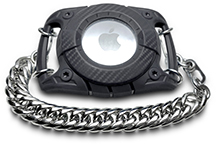
\includegraphics[width=0.35\textwidth]{images/AirT-Blk-Sm.jpg}
    \caption{Unremovable bracelet (image from \cite{bracelets}).}
    \label{img:brac}
  \end{figure}
  \item \textit{Intrusion detector}: An innovative usage can be as an intrusion detector. In a scenario where it is needed to check whether anyone is near a specific remote cabin; if an AirTag is hidden somewhere near it and someone with an iPhone passes nearby, then a notification will be sent in minutes since the intruder's device will forward to iCloud the AirTag position.
  \item \textit{Wallet tracker}: This can be the most obvious application of this kind of device. Many wallets have been developed with built-in space for the AirTag, making it easier for users to track their wallets.
  \item \textit{Supermarket shelf localizer}: An interesting application is to use it as a tracking device in a supermarket. In a scenario where an elderly person goes shopping in a very large supermarket and gets lost, an application could be developed that uses Apple’s APIs to help the user find all the shelves, using the Precision Finding offered by UWB. In the future, tablets integrated into shopping carts could be available, allowing users to find the shelves using the navigation provided in FindMy (Precision Finding).
\end{itemize}

\subsection{Mods}
After some Internet research, the author found out that the AirTag has been modified in some ways. For example, in \cite{telecomando}, A. Catley has attached the AirTag to a remote controller and powers the AirTag components from the host's battery. This could be very useful in situations where the remote controller is lost in the house; thanks to Precision Finding, the owner can easily find it again. Figure \ref{img:controller} shows the final result.
\begin{figure}[]
	\centering
	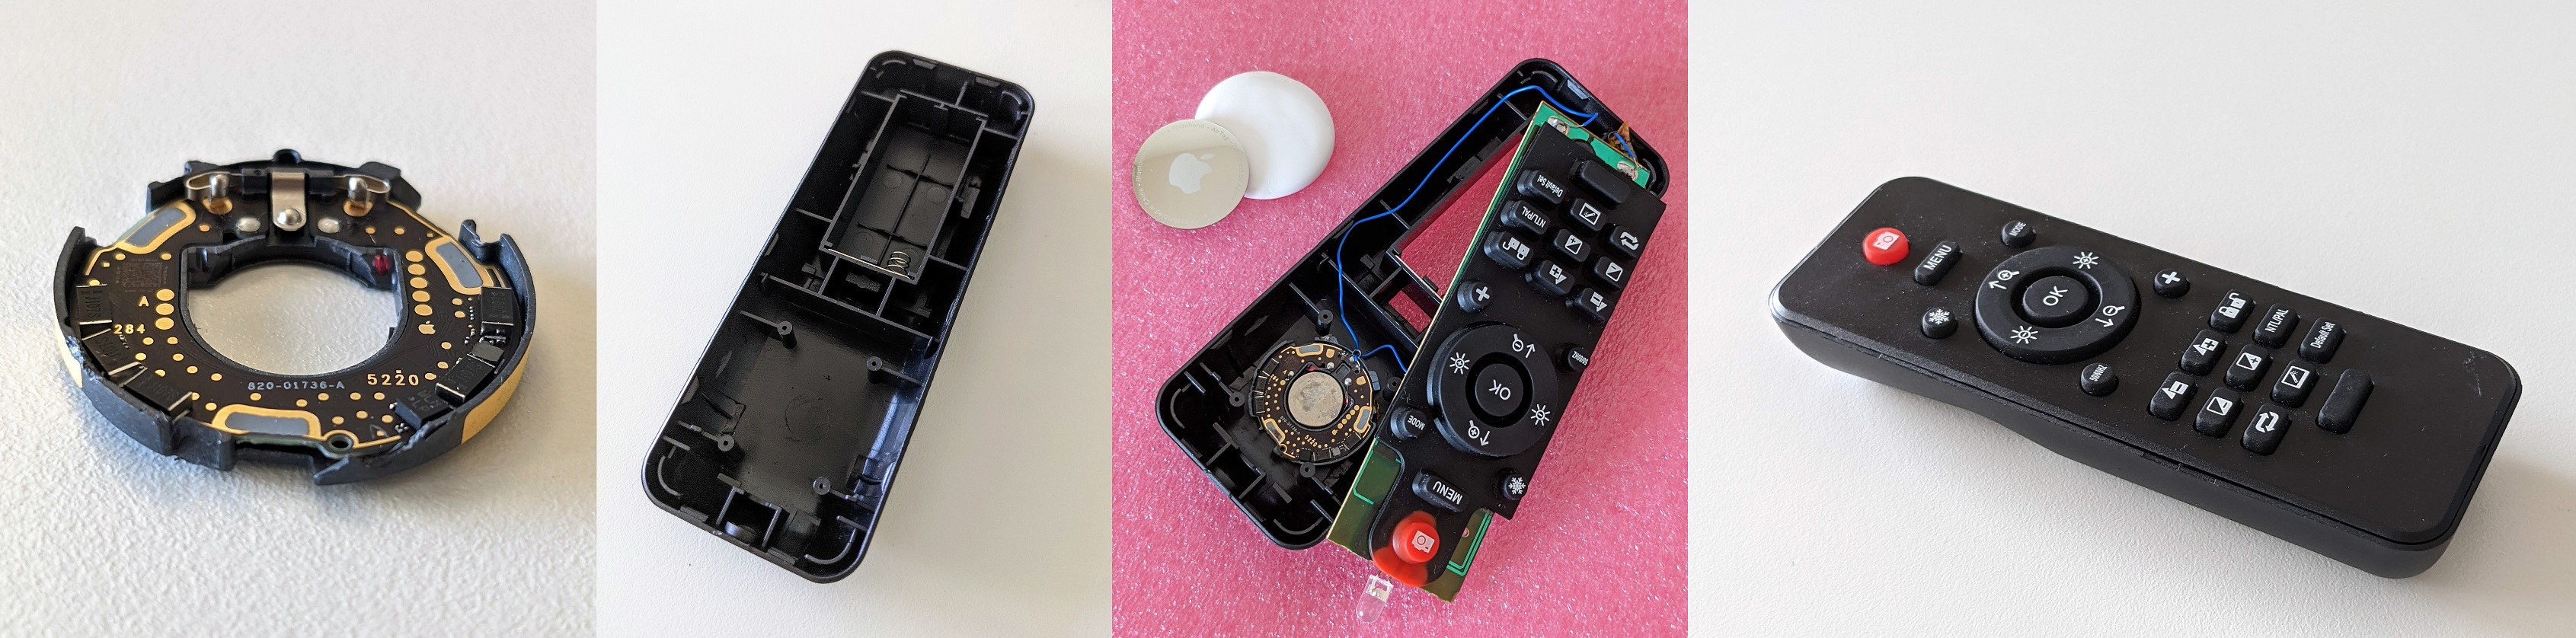
\includegraphics[width=\textwidth]{images/remote.jpg}
	\caption{AirTag inside a remote control (images from \cite{reverse}).}
	\label{img:controller}
\end{figure}


\section{Conclusion}
In conclusion, the article provides a comprehensive examination of various technological aspects. The AirTag technology and the FindMy architecture offer a smart solution to the problem of location by intelligently utilizing the worldwide network of Apple devices, and at a much lower price than the competition. Other technologies also use the same principle, but the strength of AirTag lies in the worldwide network of Apple devices. According to \cite{Lin}, Apple currently holds $29.27\%$ of the smartphone market share, which explains why the service works so well. There are numerous possibilities for the future, some of which have been discussed in Section \ref{appl}. One possible future development of this technology could be to integrate it into everyday devices to provide them with precise tracking capabilities; for example, FindMy could be integrated into shopping carts in supermarkets to locate shelves. In the future, this technology can only improve as the network of Apple devices that support both FindMy and Precision Finding continues to grow with the purchase of new iPhones (which now integrate the UWB chip). In terms of security, the vulnerabilities mentioned in Section \ref{sec:vuln} need to be addressed as user privacy is of paramount importance and a company like Apple cannot afford to ignore this issue.
\printbibliography
\nocite{*}

\end{document}